
\subsection{Sequence Diagram Use Case 1}

Det første diagram, der udarbejdes er Sekvens diagrammet for Use Case 1.
Sekvensdiagrammet er med til at give overblik over de forskellige funktioner, der skal implementeres i design og implementeringsfasen.
På sekvensdiagrammet tilføjes også States, som benyttes i State Machine Diagrammet, som kan ses senere i arktitekturen. 

\begin{figure}[H]
\centering
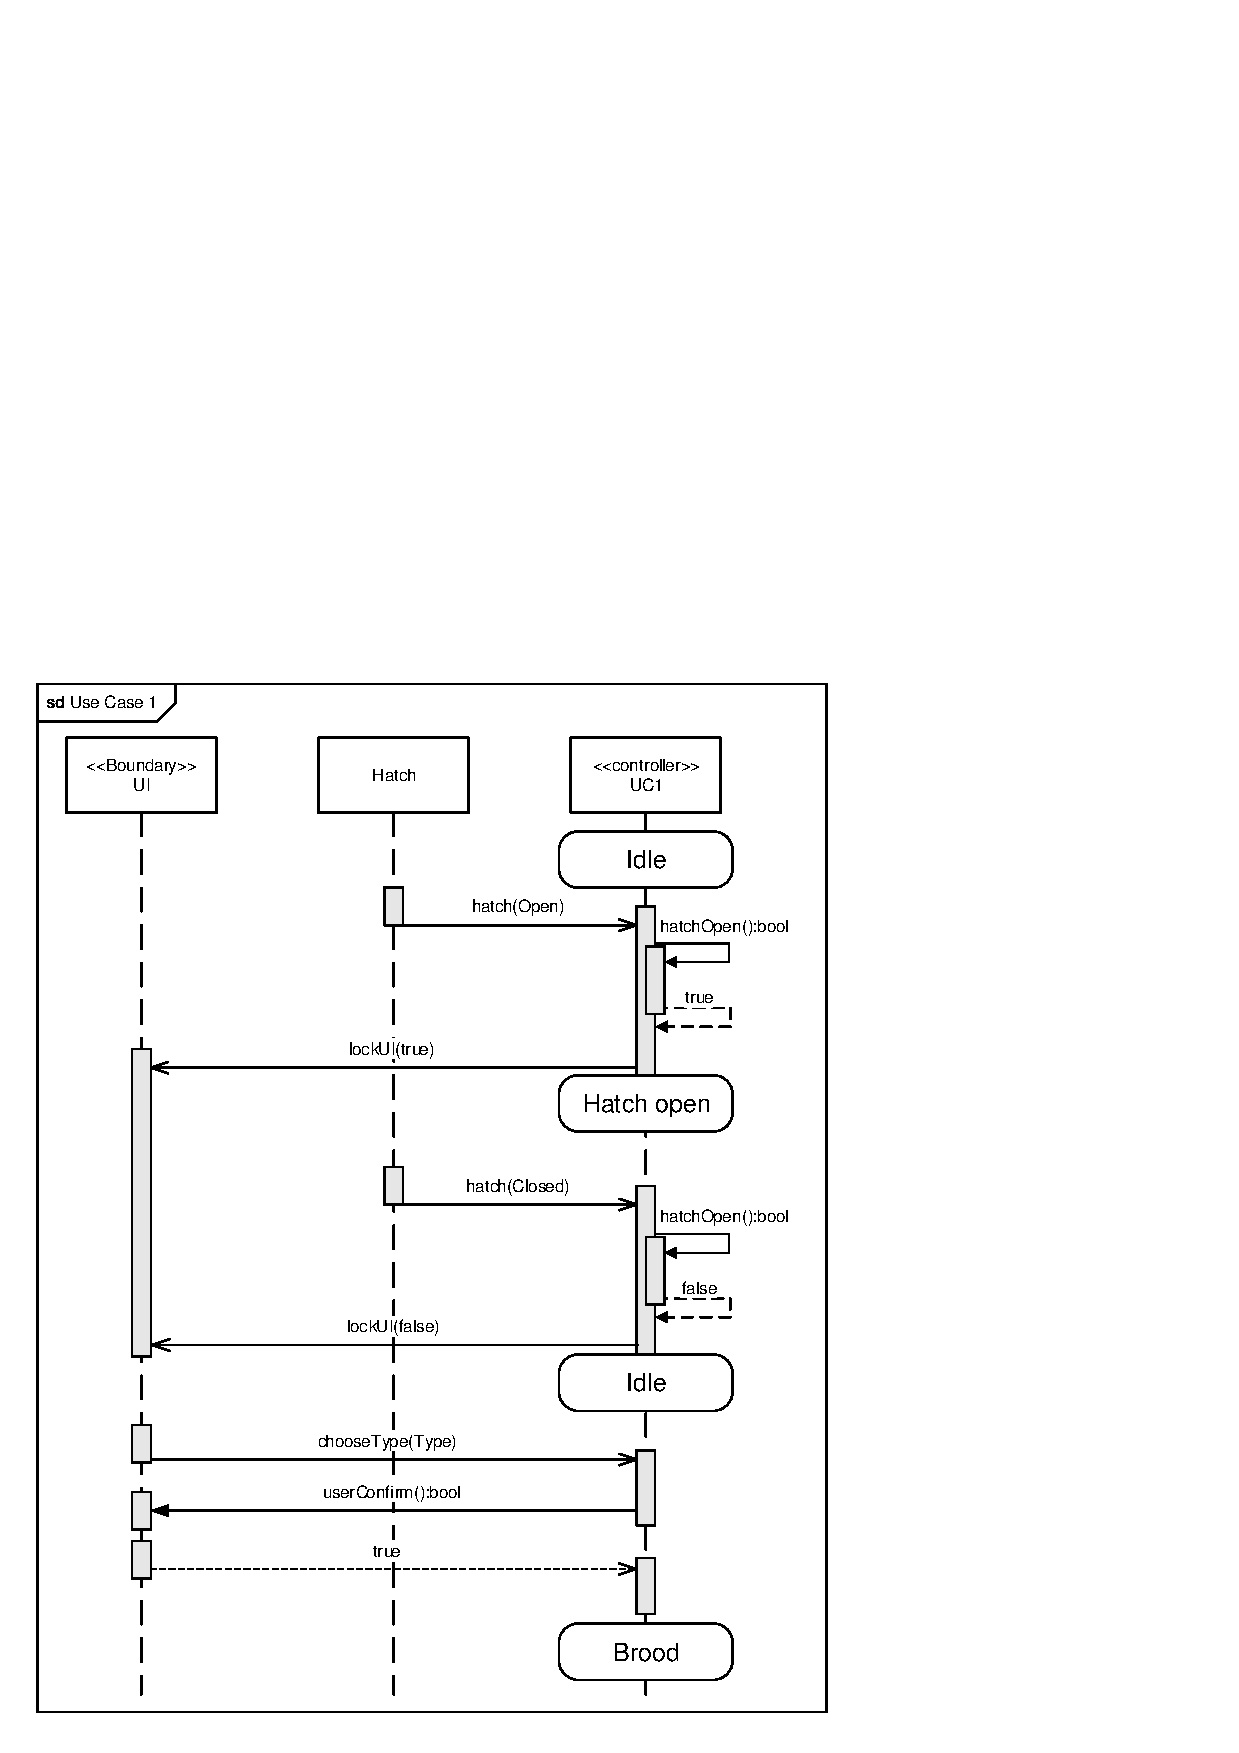
\includegraphics[page=1,width=\linewidth,viewport=07mm 08mm 139mm 180mm]{./2_systemarkitektur/diagrammer/ArkitekturDiagrammer.pdf}
\caption[Diagram]{Sequence diagram - Use Case 1}
\label{fig:SystemStateDiagram}
\end{figure}

\clearpage